\documentclass[UTF8,zihao=-4,fontset=windows]{ctexart}
\usepackage[a4paper,margin=23mm]{geometry}
\usepackage{booktabs,longtable,tabularx,array,graphicx,amsmath,xcolor,fancyhdr,float}
\usepackage[hidelinks]{hyperref}
\definecolor{ink}{HTML}{173E52}
\ctexset{section={format=\Large\bfseries\color{ink}},subsection={format=\large\bfseries\color{ink}}}
\setlength{\parskip}{5pt}
\setlength{\emergencystretch}{3em}
\renewcommand{\arraystretch}{1.16}
\pagestyle{fancy}\fancyhf{}\fancyhead[L]{\small bdd26 · 阶段报告 6}\fancyhead[R]{\small 2026 年 10 月 26 日}\fancyfoot[C]{\thepage}
\setlength{\headheight}{15pt}
\newcommand{\src}[1]{\par{\footnotesize\color{gray}本节依据：#1}\par}
\newcommand{\pp}{\text{ 个百分点}}
\title{\bfseries 从“能拟合”到“能可靠地找到”\\[8pt]\Large 核实例分割研究阶段报告 6}
\author{Xinhao Jin · Biomedical Data Design}
\date{研究范围：2026 年 10 月 13 日至 10 月 26 日\\日期与作业时间采用美国东部时间}
\begin{document}
\maketitle
\begin{abstract}
阶段报告 5 结束时，简单的事后分型与候选质量学习都没有通过预设条件。本阶段把问题进一步移到训练和实例生成过程：裁切造成的可见性变化能否用监督修复？集合查询为何丢失实例？先预测中心点、再生成掩码是否值得推进？

现有结果没有产生可以进入三划分确认的新方法，但让几个容易混淆的问题分开了。裁切敏感性真实存在，所测试的可见性监督却未能修复它；查询模型能产生一部分可用的原始掩码，却在分类保留和像素竞争后丢失很多对象；点检测可以把拟合图像记得很准，换到留出图像后仍缺少可靠的召回与精度。增加训练预算、重采样稀有类、限制骨干更新等具体办法，尚未改变这一局面。

报告按证据说明每条路线为何停止，保留已经观察到的局部正信号，也说明它们为什么不足以支持扩量。最新 P16 仍只取得一个种子的完整结果；新一轮 P17 将卷积金字塔检测器与原 UNI 检测器作独立对照，检验不同表征配方是否值得继续研究。
\end{abstract}
\begin{quote}\small\textbf{本轮核实状态：}P16 seed 19 两组已完成并核验；seed 1 仍运行。P17 真实 V100 验证 55297045 已通过；正式数组 \textbf{55297061} 于 2026 年 10 月 26 日 \textbf{09:08:19（美东时间）}单次提交，四项初始均排队。提交不代表训练完成，也不代表方法通过。\end{quote}
\newpage
{\small\tableofcontents}
\newpage

\section{本阶段改变了什么}

上一份报告主要回答“分错类别是否能靠读出已有特征来修正”。本阶段换了一个更靠前的问题：在不告诉模型真值位置的情况下，它能否先产生一组找得全、报得准的实例，再把这些实例转成可靠的分割结果？这条路径与 Dead 类问题有关，也关系到拥挤区域的实例分离和不同组织上的稳定性。Dead 沿用数据集类别名，包含凋亡和坏死相关细胞核，不等同于“凋亡”。

\subsection{哪些属于方法结果，哪些只是诊断}

本阶段使用三种口径。第一种是完整分割模型在 fold2 上的开发验证：mPQ 同时考虑实例轮廓、匹配和类别，bPQ 不区分类别，strict Dead 还惩罚缺类图像上的 Dead 误报。第二种是训练折内部按图像留出的点检测研究，衡量预测中心能否在原生图像 3 像素半径内与真值唯一匹配；它不检查掩码轮廓，因此不能当作 PQ。第三种是给定真值位置或对应关系的拟合试验，用来判断网络是否存在可拟合空间；这种帮助在实际推理时拿不到。

三种结果不直接相减。尤其不能把点召回和掩码 IoU 匹配率之间的差值称为流水线损失，也不能把训练诊断的高召回写成模型在新图像上的成绩。

\begin{table}[H]\centering\small
\begin{tabularx}{\linewidth}{p{24mm}XX}\toprule
研究部分 & 主要证据 & 目前的判断\\\midrule
可见性监督 & 受控裁切审计；四组、双种子完整训练 & 敏感性成立，所测试的监督修复未通过\\
集合查询分割 & E6/E7 完整训练；输出阶段逐对象诊断 & 配方发生全局退化，简单日程调整未救回\\
高分辨率适配 & E19 双种子对照及失败对象交集 & 单 skip 残差适配器未修复内部 Dead 召回\\
中心点检测 & P1-R1、P3--P15 的拟合/留出对照 & 高拟合未形成可靠泛化，现有配方未获扩量资格\\
最新实验 & P16 单种子完整结果；P17 独立新设计 & P16 待收齐；P17 检验卷积表示配方\\\bottomrule
\end{tabularx}
\end{table}

这里的“未通过”指未满足提前固定的全部条件，不是某个指标完全没有上涨。为了避免事后挑选有利结果，我们始终保留最初的主端点和质量约束。多个实验反复使用相同图像，失败次数也不能当成彼此独立的统计投票。

\src{阶段报告 5；10 月 15 日研究综合；E 系列 10 月 18 日复盘；P3--P15 综合。历史结果在本轮核对当前文档，未重新运行全部旧模型。}

另完成了 Inf/Conn 类别合并审计：合并空间的官方指标增约 .0519，理想分类上限差距缩小约 35.2\%。这包含合并类别本身的机械收益，不能当作标签模糊损失的估计；五类方法分数不变。

\section{可见性：发现脆弱点，不等于找到了修复办法}

\subsection{裁切审计给出了什么证据}

E4 先比较原图贴边与内部对象，再对原本完整的核施加固定裁切。修正后的结果中，按面积分层的原图贴边减内部 Dead 漏检差为 $+0.1738$，95\% 区间为 $[0.1060,0.2528]$；受控裁切的差中差为 $+0.1474$，而插值对照仅约 $-0.0006$。新截断对象中，小于 30 原生像素的碎片比至少 100 像素的对象，漏检率高 $0.8175$，区间为 $[0.7968,0.8393]$。这些结果支持继续研究裁切相关脆弱性。

这一步曾有一次重要修正：早期版本包含 train 模式推理和未按面积分层的判定。正式依据是 10 月 14 日修正后的产物，不能继续引用旧版本作为有效结论。即便修正后通过，也不能由此认定“HV 目标被置零”就是全部漏检的原因；被裁切的图像同时改变了可见面积和上下文。

\subsection{四组完整训练没有支持选择性监督修复}

随后比较 A0 原始训练、A1 裁切增强、A2 裁切增强加选择性 HV 监督、A3 更广泛的小目标监督。两种子各训练 130 轮，使用最后检查点，在原图和固定裁切图上分别评估。

\begin{table}[H]\centering\small
\begin{tabular}{lrrrr}\toprule
两种子平均变化 & mPQ & bPQ & Dead PQ & strict Dead PQ\\\midrule
A1$-$A0 & $-.005284$ & $-.006122$ & $+.037648$ & $+.008833$\\
A2$-$A0 & $-.006269$ & $-.005438$ & $+.024565$ & $-.000948$\\
A2$-$A1 & $-.000985$ & $+.000685$ & $-.013083$ & $-.009781$\\\bottomrule
\end{tabular}
\caption{fold2 原图开发结果。平均值描述两个固定种子，不能据此自行补出显著性。}
\end{table}

裁切增强 A1 的 Dead 指标确有正信号，但伴随总体分割质量下降。A2 不仅未能消除代价，较 A1 的 Dead 和 strict Dead 还在两个种子上同时下降。原图质量约束因此失败。

更直接的裁切机制检验只由 38 张图中的 116 个符合条件的 Dead 对象支持。A1$-$A2 的漏检改善在两个种子上分别为 $-.025862$ 和 $+.008621$，平均 $-.008621$，95\% 区间 $[-.040918,+.017699]$。正值才代表 A2 少漏检，实测没有达到要求。

因此，这里应保留两句话：模型对裁切敏感；所测试的选择性监督没有完成预期修复。前一句不能替后一句过关，后一句也不能推翻所有可见性训练方法。

\src{E4\_\allowbreak{}VISIBILITY\_\allowbreak{}PROBE\_\allowbreak{}2026-10-13；VISIBILITY\_\allowbreak{}SUPERVISION\_\allowbreak{}DEV 与 MECHANISM\_\allowbreak{}2026-10-15。E4 修正产物日期为 10 月 14 日。}

\section{集合查询：瓶颈出现在实例生成的整条链上}

\subsection{完整训练的退化远大于小幅种子波动}

E6 把密集分割基线 B 与查询掩码模型 Q 作匹配对照；E7 再单独将学习率衰减系数从 .85 改为 .99，检验过快衰减是否足以解释失败。各轮均为两组乘两个种子、每次 130 轮，fold1 训练、fold2 开发验证。

\begin{table}[H]\centering\small
\begin{tabular}{llrrrr}\toprule
实验 & 模型 & mPQ & bPQ & Dead PQ & 合并率\\\midrule
E6 & B 密集基线 & .481432 & .650773 & .179635 & .045363\\
E6 & Q 查询掩码 & .102699 & .192614 & .005951 & .285885\\
E7 & B 密集基线 & .472939 & .650651 & .131493 & .051209\\
E7 & Q 查询掩码 & .087958 & .169912 & .006287 & .219744\\\bottomrule
\end{tabular}
\caption{各轮两个固定种子的均值。只能与同轮匹配基线比较。}
\end{table}

Q 的五类 PQ 和全部 19 个组织的 mPQ 都低于对应 B。E6、E7 内部 Dead 的 IoU$>.5$ 匹配率变化分别为 $-.507422$ 和 $-.528340$，对应区间都完全低于零。减慢衰减没有恢复基本实例质量。成本检验虽然通过，也不足以使这样的质量损失变得可接受。

这不等同于“模型完全看不到核”。E6 中，内部 Dead 的 IoU 处在 .1 到 .5 之间的比例从约 9.99\% 上升到 55.60\%。大量对象有部分重叠，却没有形成合格实例，涉及定位、轮廓及实例分离，不能统称为完全漏检。

\subsection{原始掩码为什么没成为最终实例}

对 E7 的同一批 16 张训练图、331 个目标，进一步追踪所有查询中的最佳匹配，而非只盯着训练时分配给该目标的查询。

\begin{figure}[H]\centering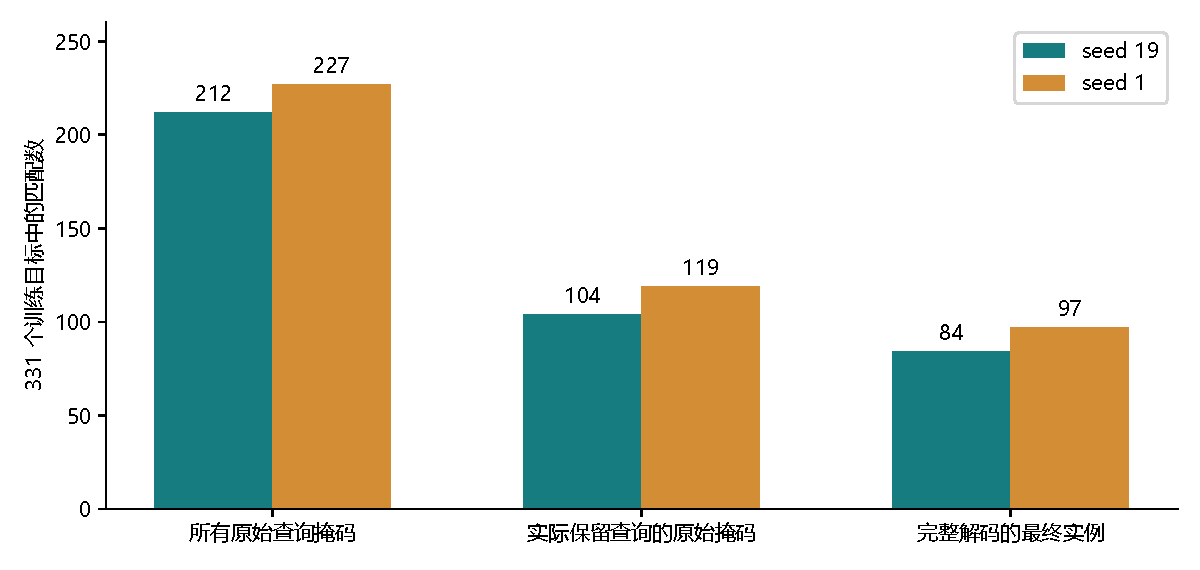
\includegraphics[width=\linewidth]{figs/query_attrition.pdf}
\caption{E7 的固定训练批次诊断。所有原始掩码阶段使用真值寻找最佳重叠，是诊断上界，不是部署成绩。}
\end{figure}

seed 19 从 212 个原始达标对象降到保留查询中的 104 个，完整解码后剩 84 个；seed 1 为 227、119、97。原始掩码到查询保留，两种子都损失 108/331，即 32.63 个百分点；像素竞争后的净损失又约 6 个百分点。直接降低置信度阈值不能解决背景 argmax 的拒绝，而且原始掩码上界本身也只有 64\%--69\%。

这说明应把“学到掩码”“判断哪个查询是对象”“解决重叠竞争”分别检查，不能只凭训练损失下降或几张看起来不错的掩码扩大训练。

\src{SET\_\allowbreak{}MASK\_\allowbreak{}E6\_\allowbreak{}DEV\_\allowbreak{}2026-10-16；SET\_\allowbreak{}MASK\_\allowbreak{}E7\_\allowbreak{}DEV\_\allowbreak{}2026-10-17。}

\section{小规模诊断把“可表示”和“可推理”分开}

E8--E18 没有直接继续扩大完整模型，而是针对分类读出、查询初始化、注意力、监督和对象对应关系做训练内诊断。它们的价值在于排除具体修补方案，也暴露了一种容易误判的正结果：给了真值帮助以后可以拟合，不代表正常推理时能自己找到对象。

\begin{longtable}{p{20mm}p{45mm}p{80mm}}
\toprule 实验 & 改变或检查的部分 & 结果及其边界\\\midrule\endhead
E8 & 冻结特征，仅调整分类读出 & 前景拟合准确率约 95\%--98\%，但留出图像的前景判断下降，未通过分配条件。分类读出改善并未转成可靠实例集合。\\
E9 & 用局部内容初始化查询 & 内部 Dead 的小幅点估计改善伴随精度下降；两种子均未通过，不能据此直接扩训练。\\
E10 & 预测掩码限制注意力 & 两种子的内部 Dead 变化为 $-.067511/+.008439$，总体召回也下降；未解决原问题。\\
E11 & 四阶段辅助监督 & 原分配条件和独立 A0 约束均失败，停止该固定配方。\\
E12/E13 & 真值辅助的自由系数或稳定投影 & E12 两种子拟合 Dead 为 86.32\%/87.37\%，证明有限条件下可拟合；E13 冻结投影后质量条件仍失败。\\
E14 & 精确的原生匹配 & 匹配本身完成，但实例分配和 A0 约束仍未通过，不能把更精确的匹配等同于方法有效。\\
E15/E16 & 真值点读出及点条件掩码 & E16 拟合图像 Dead 为 84.21\%/80.26\%，本轮读出留出图像为 31.58\%/42.11\%；冻结 E7 已见过这些图，不是整模型独立泛化证据。\\
E17 & 预测稀疏点产生候选 & 固定训练诊断中没有输出候选，当前配方失败。\\
E18 & 稠密投票产生候选 & 候选过多，最终实例推理的审计精度约 3.5\%--3.7\%；这不是后续 P3 的半径 3 像素点指标。\\\bottomrule
\end{longtable}

这些诊断重复使用了很小的队列，既不是独立验证，也不是对查询或点方法整个家族的否证。E6/E7 已有完整训练负结果，不能简单说“只需多训”；E12/E16 的正结果又说明“完全没有表征能力”同样过于绝对。后续研究因此转向更基本的条件：先检验实际预测候选的召回、精度和跨图像泛化，再决定是否接入掩码模型。

\src{QUERY\_\allowbreak{}MECHANISM；LOCAL\_\allowbreak{}QUERY\_\allowbreak{}E9；MASKED\_\allowbreak{}QUERY\_\allowbreak{}E10；AUX\_\allowbreak{}QUERY\_\allowbreak{}E11；FREE\_\allowbreak{}MASK\_\allowbreak{}E12；STABLE\_\allowbreak{}MASK\_\allowbreak{}E13；NATIVE\_\allowbreak{}MATCH\_\allowbreak{}E14；POINT\_\allowbreak{}READOUT\_\allowbreak{}E15；GT\_\allowbreak{}POINT\_\allowbreak{}MASK\_\allowbreak{}E16；E17/E18 诊断及 10 月 17 日综合。}

\section{门控与高分辨率适配：局部正信号为何没有完成主目标}

E5 的门控融合曾让 official Dead PQ 平均提高 .017897、strict Dead PQ 提高 .014202，却没有稳定改善内部 Dead 的几何匹配：平均变化 $-.003374$，95\% 区间 $[-.014273,+.007486]$。匹配对象的构成和分型质量发生了变化，不能把 PQ 上涨全部归为缺类规则的漏洞，也不能由此宣称找回了漏检。由于事先选定的主目标未通过，这个配方没有继续扩量。

E19 在 CellViT-UNI 最细的解码 skip 上加入零初始化的 CNN 残差分支。四次完整训练之后，内部 Dead 匹配率平均变化为 $-.008097$，95\% 区间 $[-.022566,+.007378]$；official Dead PQ 平均下降 .001774。strict Dead PQ 虽提高 .008128，主目标仍未通过。

这不是对完整多尺度适配方法的复现，也不能推翻早期放大工作分辨率时观察到的现象；它否定的是这个插入点、结构和预算下的具体配方。

\subsection{失败交集揭示了哪些对象值得继续研究}

对同一 741 个内部 Dead 对象，四个模型共同未达到 IoU$>.5$ 的有 233 个，占 31.44\%；四个模型始终 IoU$<.1$ 的有 149 个，占 20.11\%。前者包含粗略定位但形状不合格，不能全部称为完全漏检。

在 233 个持续未匹配对象中，176 个面积小于 100 像素，面积中位数为 64。四模型的匹配并集为 508/741，比最强单模型的 471 个只多 37 个。这一并集利用真值判断，不处理误报和冲突，不能当成可部署集成模型；它只是说明盲目融合这些预测的剩余覆盖空间有限。

\begin{table}[H]\centering\small
\begin{tabular}{lrrr}\toprule
由训练折定义的面积组 & 训练对象数 & 开发对象数 & 四模型共同未匹配\\\midrule
$<67$ & 200 & 179 & 123（68.7\%）\\
67--102 & 196 & 209 & 55（26.3\%）\\
103--157 & 204 & 189 & 20（10.6\%）\\
$\ge158$ & 201 & 164 & 35（21.3\%）\\\bottomrule
\end{tabular}
\caption{固定对象的描述性分组。面积切点来自训练折，未根据开发失败对象重新选切点。}
\end{table}

面积和局部对比度的 16 个组合格在训练折都有对象支持，训练/开发边际中位数也接近。这排除了简单的“训练中根本没有这种尺寸或对比度”的解释，却不能排除组织、外观和未知患者因素联合产生的分布差异。小尺寸与失败关联很强，但大对象也有持续失败，因此没有证据把尺寸认定为唯一原因。

组织支持尤其不均衡：这批内部 Dead 中 Lung 占 535/741，Colon 83 个；这与全数据 Dead 标签中 Lung 占 59.5\% 是不同分母。七个组织没有 Dead 标签，更不能把没有可评对象写成性能很好。

\src{FUSION\_GATING\_DEV；HIRES\_\allowbreak{}ADAPTER\_\allowbreak{}E19\_\allowbreak{}DEV；E\_\allowbreak{}SERIES\_\allowbreak{}REVIEW 与 RESEARCH\_\allowbreak{}DECISION\_\allowbreak{}CELLVIT\_\allowbreak{}PMNET\_\allowbreak{}2026-10-18；TISSUE\_\allowbreak{}CLASS\_\allowbreak{}AUDIT\_\allowbreak{}2026-10-15。}

\section{中心点路线：学会训练图像，仍没有学会可靠迁移}

\subsection{P1-R1 排除了“原来只是没训够”的充分解释}

最初的冻结特征点头训练不足时没有产生候选。按提前约定的训练损失停止规则延长后，两个种子分别训练到 55/60 轮，训练内召回达到约 94\%--98\%，精度约 99.9\%。但 fold2 内部 Dead 点召回只有 .40756/.39541，低于固定 NP-component 参考的 .74899，两个种子的差值区间都低于零。

补足拟合预算没有使它可靠泛化，因此原 P1 到 P2 的前提没有满足。这里的 NP-component 是点候选参考，不是掩码 IoU 或正式 PQ，不能把两者混成模型排名。

\subsection{P3 把表征适配和训练增强分别检验}

P3 在 fold1 内固定划分 2,134 张拟合图像与 522 张审计图像。审计集只有 11 张内部 Dead 阳性图、145 个内部 Dead，其中 Lung 和 Colon 合计 116 个。所有组都使用原图中心目标和固定解码，比较冻结/适配 UNI 与无/有增强的四种组合，各做两个种子、130 轮训练。

\begin{table}[H]\centering\small
\begin{tabular}{lrrrr}\toprule
组别 & 拟合召回 & 审计召回 & 审计精度 & 审计 Dead 召回\\\midrule
F0 冻结、无增强 & .999922 & .442776 & .706998 & .351724\\
F1 冻结、有增强 & .538848 & .428857 & .815171 & .396552\\
T0 适配、无增强 & .999833 & .509918 & .724614 & .375862\\
T1 适配、有增强 & .977035 & .588939 & .692705 & .437931\\\bottomrule
\end{tabular}
\caption{P3 两个固定种子的算术均值，均为点匹配。}
\end{table}

无增强时可以几乎记住拟合图像；有增强时，冻结表征组本身就难以拟合，适配后拟合大幅恢复。T1 相对 F1 的总体审计召回确实提高了约 16 个百分点，但精度下降约 12.25 个百分点。内部 Dead 的提升在两个种子上为 6.90 和 1.38 个百分点，区间都跨零。召回、精度和稳定性不能只选其中一项。

\subsection{通过条件为何不能事后放宽}

原条件要求处理组在两个种子中分别满足：内部 Dead 召回至少 .60、较对应对照提高至少 .05、原组织分层图像 bootstrap 的区间下界大于零；唯一匹配精度至少 .75，且不得比对照低超过 .02；总体召回不得低超过 .02，并满足样本支持与非退化条件。全部条件同时成立，才有理由讨论下一步。

这个标准并不声称具有理想的统计功效。11 张阳性图的支持本来就很少，多轮选题又反复看同一个审计集。它的作用是约束研究决策，避免把偶然的单种子上涨当成扩量依据。

\src{P1R1\_\allowbreak{}RESULT\_\allowbreak{}2026-10-18；PROPOSAL\_\allowbreak{}P3\_\allowbreak{}PHASE\_\allowbreak{}A\_\allowbreak{}2026-10-20；原 admission 实现。}

\section{P4--P15：哪些尝试已经排除，哪些判断仍然不能下}

后续各轮保留固定队列、种子、130 轮、最后检查点及通过条件，每轮只引入一个固定配方，并重新训练本轮对照。表中数字是本轮处理组减去本轮对照；不得把不同轮的处理组直接排名，也不能将种子当成独立患者样本。

\begin{table}[H]\centering\small
\begin{tabularx}{\linewidth}{p{12mm}Xrr}\toprule
实验 & 固定改变 & seed 19 & seed 1\\\midrule
P4 & 稠密前景辅助 BCE & $-.027586$ & $+.006897$\\
P5 & 等容量的原生网格细化 & $.000000$ & $-.006897$\\
P6 & 放宽 Gaussian 邻域的负损失抑制 & $+.020690$ & $+.020690$\\
P7 & 训练期 RGB 通道扰动 & $+.034483$ & $-.013793$\\
P8 & 按图像内对象数归一化损失 & $-.034483$ & $-.048276$\\
P9 & Dead 中心正损失权重 4 & $+.006897$ & $+.048276$\\
P10 & 只适配最后 4 层，而非最后 12 层 & $+.027586$ & $-.013793$\\
P11 & 重分配精确中心的正 focal 质量 & $+.041379$ & $.000000$\\
P12 & 解码 stem 后通道 dropout .2 & $-.034483$ & $-.027586$\\
P13 & 25\% 训练位置替换为稀有类阳性图 & $-.137931$ & $-.048276$\\
P14 & 编码器学习率 $10^{-5}$ 改为 $10^{-6}$ & $-.068966$ & $-.089655$\\
P15 & 训练整数平移 $\pm16$，白色填补 & $-.193103$ & $-.089655$\\\bottomrule
\end{tabularx}
\caption{内部 Dead 点召回变化。P4--P15 的原通过条件均未满足。}
\end{table}

\begin{figure}[H]\centering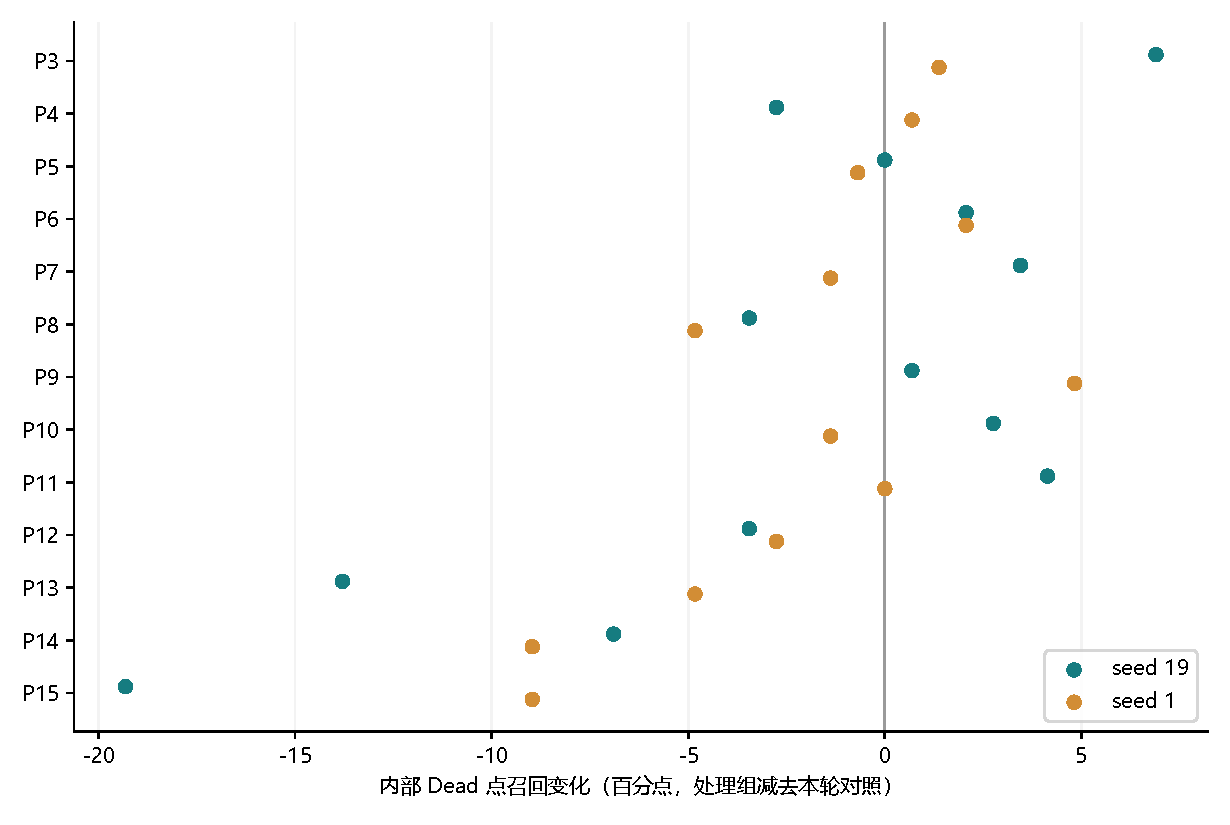
\includegraphics[width=.92\linewidth]{figs/proposal_deltas.pdf}
\caption{P3--P15 按时间排列。P3 是 T1$-$F1，其余是各轮处理$-$新对照。图仅展示点估计，不是显著性或超参数优劣排名。}
\end{figure}

\subsection{负结果至少有三种不同形态}

第一种是\textbf{拟合很好、审计不够好}。P13 更频繁展示稀有类阳性图后，拟合 Dead 召回为 .998476/1，审计却只有 .351724/.358621。增加稀有类图像的训练次数并未在这套配方中带来迁移，不能把失败简单归为“样本没看够”。

第二种是\textbf{减少适配不等于提高泛化}。只训练更少骨干层、加 dropout、减小骨干学习率都没有通过。P14 的精度提高，却伴随总体召回下降约 8.83/12.01 个百分点。单看精度会误以为模型变可靠，实际上它也少报了很多对象。

第三种是\textbf{增强后连拟合任务也明显变难}。P15 在无增强的拟合图像上，总体召回从约 .978 降到 .470，内部 Dead 从约 .952 降到 .45。它与“已经拟合但没迁移”的 P13 不同。白边、部分可见核、每轮约 9.94\% 中心目标被移出画面，以及位置不变性要求一起变化，不能由这一轮单独归因于位置编码。

P15 的审计精度从 .692/.698 提高到 .865/.863，但候选数从 10,469/10,428 降到 5,498/5,397，唯一匹配数也从 7,241/7,280 降到 4,758/4,657。两种子内部 Dead 的差值区间均完全低于零。这是覆盖率大幅下降的明确负结果，不能把更高精度写成整体改善。512 候选上限未触发，也不支持“候选被 cap 截断”这一解释。

这些结果已经足以停止扩展上述固定配方。它们没有证明所有增强、重加权、卷积或点检测方法都无效，更没有定位一个适用于全部实验的单一失败原因。

\src{P4--P15 各轮结果文档；PROPOSAL\_\allowbreak{}PROGRESS\_\allowbreak{}2026-10-26。本轮对汇总表逐行和当前原始结果文档交叉核对，未重新哈希所有历史大检查点。}

\section{最新结果与下一轮：先保留结论边界，再推进实验}

\subsection{P16：完整 Gaussian 回归，目前只报告一个种子}

原 focal 损失只把精确中心作为正点，Gaussian 周边值用于减轻附近负损失。P16 保留目标几何，处理组直接最小化 sigmoid 输出与 Gaussian 的平方误差总和，再除以有效批次对象数；系数固定为 1。它同时改变梯度、背景权重和损失尺度，因此不能将结果解释为单独证明了 Gaussian 周边监督或概率校准的作用。

截至本轮首批回收，seed 19 两组已完成 130 轮，SLURM 均为 COMPLETED/0:0。18 个小结果文件的大小和 SHA256 与保存清单一致，401 个封存源码文件逐项核验；拟合/审计图像身份、130 轮日志及逐图聚合结果通过核对。

\begin{table}[H]\centering\small
\begin{tabular}{lrr}\toprule
seed 19 & 原 focal 对照 C & Gaussian 回归 R\\\midrule
拟合总体召回 & .980007 & .872135\\
拟合内部 Dead 召回 & .961890 & .846037\\
审计总体召回 & .598041 & .602531\\
审计唯一匹配精度 & .694079 & .701149\\
审计内部 Dead 召回 & .482759 & .517241\\\bottomrule
\end{tabular}
\end{table}

Dead 提高 $+.034483$，按原始 1,000 次组织分层图像抽样重算的 95\% 区间为 $[-.034091,+.131144]$。提高对应多匹配 5 个对象；原始单种子条件仍失败：绝对召回不足 .60、增益不足 .05、区间跨零、精度不足 .75。

seed 1 在首批回收时仍运行，C/R 分别为第 70/58 轮。本报告不据此虚构双种子均值或完整收尾结论。即使另一个种子较好，也不能覆盖已完成种子未通过的条件。大型检查点本轮未独立重哈希，外部归档仍待安排。

\subsection{P17：把卷积表示作为独立配方检验}

新实验在 P16 的 seed 1 完成之前固定设计，不依赖其尚未完成的结果。对照 C 使用原 UNI 检测器；K 从头训练三阶段卷积金字塔，宽度为 32/64/128，融合多尺度特征后输出原生中心热图。K 不叠加查询、掩码、稀有类重采样或额外监督。

两组保留相同的拟合/审计队列、原 focal 损失、Gaussian 目标、增强、固定解码和通过条件。K 的全部参数学习率为 $3\times10^{-4}$；C 仍使用头部 $3\times10^{-4}$、骨干 $10^{-5}$。因此这是一套架构、初始化、预训练和优化共同变化的配方比较，不是纯粹“局部性”的因果实验。GroupNorm 还使用空间统计，K 也不是严格有限感受野的局部算子。

这轮要回答的实践问题很具体：换成一个从头训练的卷积表示，在原预算内是否值得继续？若失败，就关闭这个宽度、日程与损失组合，不扩宽度、种子、阈值或训练轮数；若通过，也只支持讨论下一份验证方案，不自动进入掩码或三划分确认。

\par\textbf{实际验证与提交。}V100 验证作业 55297045 已于 exp-7-59 完成，状态 COMPLETED/0:0，耗时 6 分 12 秒，291 项节点检查通过。两个种子的原对照初始化及两步完整梯度、参数、AdamW、随机状态与 P3 一致；K 的三个卷积阶段、融合头和输出层均有第二步非零梯度与更新，且排除了纯权重衰减。AMP、最后/最终检查点重载、来源与数据身份、严格 readiness 均通过。25 个小证据文件回收时核验大小及 SHA256。\par 加入 1.5 倍余量的 130 轮时间外推为 C 6.95 小时、K 4.77 小时；训练峰值显存约 4.07/0.35 GiB。这是外推，不是完工保证。正式数组 \textbf{55297061} 于 \textbf{09:08:19 EDT} 单次提交，依次 C19/K19/C1/K1，并发上限 2；每项 1 V100、4 CPU、32 GiB、12 小时，gpu-shared / gpu-shared-normal，账户 jhu159，Lustre，禁用自动 requeue。正式预算上限 48 GPU 小时，验证另限 0.5 GPU 小时。训练来源 \texttt{5a7e85b}，407 文件源码封存；提交时四项均排队。

\section{研究推进与算力迁移}

近期正式训练已经迁移到 Expanse。迁移不只是把脚本提交出去：最初的数据副本包含 420 个文件、约 8.10 GB，曾在计算节点核验全部大小和哈希；大文件通过官方 Globus 搬运。后续各轮复用这份数据、UNI 权重和固定环境，分别封存源码、保存配置与提交收据。P3 迁移前因源盘空间保护停止的运行也在保留原检查点后完成，未重新计算已完成的六项。

本轮实时检查中，LM1/LM2 没有本项目训练进程；LM1 根分区无可用空间、项目盘约余 11 GB，LM2 根分区约余 784 MB、项目盘约余 1.9 GB。因此没有在那里增加训练或回收大型检查点。Expanse 账户可用额度、GPU 分区权限及个人/项目配额已核实。原有无关作业完整保留。

P17 沿用同一持久执行通道和现有 Expanse ControlMaster，未新增认证连接或改变代理。每次提交使用独占创建的标记，记录作业 ID；结果未知时查收据和调度记录，不重复运行提交脚本。验证计算都通过 SLURM，在登录节点只做轻量检查与提交。

今天已将 P13--P16 及此前审查修正合并发布到 master，基准提交为 \texttt{f67ce20}；当时完整 CPU 回归为 828 项通过、3 项跳过。P17 在独立分支实施，本轮最终完整 CPU 回归为 861 项通过、3 项跳过（19,073 条旧依赖弃用警告），proposal 与节点专项均为 291 项通过。不同计数对应不同版本或检查范围，原回执均保留。

\section{当前能下的判断，以及还缺什么}

本阶段最扎实的进展，是把“识别不到”拆成了可检查的环节，而不是得到一个新的最高分。裁切审计与监督修复之间、原始查询掩码与最终实例之间、拟合图像与留出图像之间，都出现了明确落差。继续研究必须针对其中某个可区分的问题，不能把已经失败的模块重新堆在一起就宣称提出了新方法。

也不能把连续负结果写成问题已经无解。E19 的持续失败对象与小尺寸有关，但不是唯一尺寸机制；训练折的粗粒度支持存在，不代表联合分布充分覆盖；点检测的高拟合说明能记住图像，不说明它学到了可迁移的核外观。专家评审尚不可用，检测器共识也仍不能替代生物学裁定。

下一步先完成 P16 两个未结束运行的收尾核验，保留原判定。P17 完成后同样先核对 130 轮、来源、输入、配置和保存清单，再按两个种子分别判断。只有真实预测候选在召回与精度上同时成立，才有必要讨论掩码头和联合训练。没有通过时，优先记录失败模式和停止理由，而不是继续在同一批 11 张阳性图上放大参数菜单。

最终研究报告还需要明确保留以下限制：fold2 与 fold1 内部审计集多次复用；图像不等于独立患者；bootstrap 区间条件于固定模型和现有图像，并不覆盖训练种子总体；Dead 标签在组织间分布不均；本阶段没有新的官方三划分测试成绩。阶段报告 5 的人类专家评审义务也没有因技术实验变多而消失。

\clearpage
\appendix
\section{证据索引与复核范围}

本报告的历史数字依据 LM1 当前研究文档和各轮收尾记录，属于文档与已保存证据的综合，不声称重新评估了全部旧模型。P16 seed 19 则在本轮回收到逐图记录后重新聚合、重放原 bootstrap，核对了图像队列和 130 轮日志。来源文本摘要哈希及新数字保存在随附 \texttt{verified\_\allowbreak{}numbers.json}。

\begin{enumerate}
\item 前阶段边界：\texttt{docs/report/stage\_\allowbreak{}report\_\allowbreak{}5/README.md}，实验止于 10 月 12 日，报告发布于 10 月 13 日。
\item 可见性：\texttt{E4\_\allowbreak{}VISIBILITY\_\allowbreak{}PROBE}、\texttt{VISIBILITY\_\allowbreak{}SUPERVISION\_\allowbreak{}DEV}、\texttt{VISIBILITY\_\allowbreak{}SUPERVISION\_\allowbreak{}MECHANISM}，均位于 \texttt{docs/results/}。
\item 查询路线：\texttt{SET\_\allowbreak{}MASK\_\allowbreak{}E6\_\allowbreak{}DEV}、\texttt{SET\_\allowbreak{}MASK\_\allowbreak{}E7\_\allowbreak{}DEV}、\texttt{QUERY\_\allowbreak{}POINT\_\allowbreak{}CLOSEOUT\_\allowbreak{}E7\_\allowbreak{}E18} 及各训练内诊断。
\item 小对象与组织：\texttt{HIRES\_\allowbreak{}ADAPTER\_\allowbreak{}E19\_\allowbreak{}DEV}、\texttt{E\_\allowbreak{}SERIES\_\allowbreak{}REVIEW}、\texttt{RESEARCH\_\allowbreak{}DECISION\_\allowbreak{}CELLVIT\_\allowbreak{}PMNET}、\texttt{TISSUE\_\allowbreak{}CLASS\_\allowbreak{}AUDIT}。
\item 点检测：\texttt{P1R1\_\allowbreak{}RESULT}、\texttt{PROPOSAL\_\allowbreak{}P3\_\allowbreak{}PHASE\_\allowbreak{}A}、P4--P15 各轮结果、\texttt{PROPOSAL\_\allowbreak{}PROGRESS\_\allowbreak{}2026-10-26}。
\item 本轮：P16 小文件回收包、原保存清单、P17 冻结设计、291 项专项日志、真实 V100 验证及正式提交收据。机器路径、PID 与连接证据仅存 ignored ops，不把历史 PID 当作后续操作依据。
\end{enumerate}

本轮提交遵循\href{https://www.sdsc.edu/systems/expanse/user_guide.html}{SDSC Expanse 用户指南}并结合实时账户、分区与配额查询。数据、权重、预测和检查点保留原件，外部大产物归档尚未完成。本报告不包含新的文献排名或未经核实的最佳性能主张。
\end{document}
